\documentclass[conference]{IEEEtran}
%\IEEEoverridecommandlockouts
% The preceding line is only needed to identify funding in the first footnote. If that is unneeded, please comment it out.
\usepackage{cite}
\usepackage{amsmath,amssymb,amsfonts}
\usepackage{algorithmic}
\usepackage{graphicx}
\usepackage{textcomp}
\usepackage{xcolor}
\usepackage{apacite}
\usepackage{tikz}
\usetikzlibrary{shapes,positioning,calc}
\colorlet{lightgray}{gray!20}


\def\BibTeX{{\rm B\kern-.05em{\sc i\kern-.025em b}\kern-.08em
    T\kern-.1667em\lower.7ex\hbox{E}\kern-.125emX}}
\begin{document}

\title{Analyzing the Ethereum Blockchain}


\author{\IEEEauthorblockN{Christin Sauerbier}
\IEEEauthorblockA{
\textit{Humboldt University Berlin}\\
Berlin, Germany \\
christin.sauerbier@outlook.com}
\and
\IEEEauthorblockN{Roman Proskalovich}
\IEEEauthorblockA{
\textit{Humboldt University Berlin}\\
Berlin, Germany \\
romanarion@gmail.​com}
\and
\IEEEauthorblockN{Thomas Siskos}
\IEEEauthorblockA{
\textit{Humboldt University Berlin}\\
Berlin, Germany \\
thomas.siskos@hu-berlin.de}
}

\begin{abstract}
In the explorative study we investigate the Ethereum blockchain,  a decentralized crypto technology and a platform used for decentralized applications and currency transactions. 
The analysis covered 6 months of data, including transaction and economic data scraped from the Ethereum platform. 
The objective is to get closer insights into the Ethereum economy and find patterns in the data.
The study reveals information about the main senders and receivers during the analyzed period and the underlying business processes, plus information about the network design and potential security issues. 
Furthermore, we scrutinize certain consequences of the Ethereum hard fork that occured in 2016.
For the graph analysis the so called \emph{Small World Phenomenon} could not be confirmed for the whole network, but for subgraphs it holds true.
\end{abstract}

\begin{IEEEkeywords}

\maketitle

\end{IEEEkeywords}

\section{Introduction}
With the Introduction of Bitcoin in 2008, a signifikant new currency was brought into life.
It is based on a peer to peer network which gives the opportunity to cancel out intermediaries within money transfers, through a decentralized verification process.
With that knowledge the idea was born to use such a technology to run decentralized applications on such a platform.
Ethereum can provide that and is now the second largest cryptocurrency after Bitcoin in terms of market capitalization. []

This paper is supposed to perform an explorative study on the Ethereum blockchain. 
The idea is to replicate what Lischke and Fabian did and transfer it to another crypto technology the Ethereum Blockchain. 
They used the address spaces and transaction history of the Bitcoin blockchain and added off-set network data to get more insights about the bitcoin economy. 
The period analysed included the first four years of the bitcoin existence. 
They were able to combine off-set network data and transaction data to get good statements about the business categories the currency is used for.

This paper is structured as follows. 
Section \ref{ethereum-theory} and \ref{ethereum-blockchain} are dedicated to the basics of Ethereum and how it got evolved from the bitcoin currency, as well as the technology behind it, respectively. 
As we replicate a paper about the bitcoin blockchain [Fabian, 2016] we also compare the Ethereum blockchain with the bitcoin blockchain. We follow this by a brief literature review in section \ref{literature-review}.


After that the reader got a proper foundation that we can dive into the underlying methodology in section \ref{methods}. 
The focus here lies mainly on how we obtained our dataset in subsection \ref{methods-data-preparation} and an overview of the methods used during graph analysis in subsection \ref{methods-graph-analysis}. 
Moving onward we present our findings in section \ref{findings}, where we describe the outcome of our methods for data aquiration in subsection \ref{findings-data-preparation}, structure them using traditional statistical methods in subsection \ref{findings-descriptive} and graph analysis in subsection \ref{findings-graph-analysis}.
Finally, section \ref{conclusion} concludes the article and discusses the outlook we received during our analysis. 
We also want to use this part to discuss what are the main differences to the former paper about the bitcoin blockchain and give an idea about future work. 


\section{Literature Review}
This paper is inspired by the study of the Bitcoin transactions network performed by \cite{lischke2016analyzing}.
There, the authors examine the data for the first 4 years of the cryptocurrency with a goal of getting insights about the underlying economy and its evolution.
They also apply a number of network metrics in order to identify major nodes, clusters, and verify whether the small world phenomenon exists for the Bitcoin network.

\begin{figure*}[ht]
  \centering
  \begin{subfigure}[b]{0.49\linewidth}
    \includegraphics[width=\linewidth]{figures/search.png}
    \caption{Broad and narrow search for articles.}
    \label{fig:search_types}
  \end{subfigure}
  \begin{subfigure}[b]{0.49\linewidth}
    \includegraphics[width=\linewidth]{figures/narrow_search.png}
    \caption{Articles with a combination of keywords in the title.}
    \label{fig:narrow_search}
  \end{subfigure}
  \caption{Results of Google Scholar search for articles.}
  \label{fig:search}
\end{figure*}

The main difference of our research is that it targets Ethereum cryptocurrency.
We replicate some of the approaches suggested in \cite{lischke2016analyzing} and adopt the others or come up with new approaches due to the differences in the cryptocurrencies' design and supporting infrastructure.
More details on this are given in the Methodology section.

To make our analysis grounded on the previous Ethereum research, benefit from findings and approaches described by other authors, have an opportunity to compare our findings to previously obtained results and potentially identify blank spots in the previous studies we conduct a literature research. 

As Ethereum was introduced only in 2013 the literature landscape is relatively scarce.
Most information is not peer-reviewed and published on various blog-platforms, forums and wiki-resources.
This does not necessarily imply pure quality.
However, we decided to use those publications only as a source of background information.
Instead, the focus was made on publications that can be found using Google Scholar web search engine that indexes the full text scholarly literature.

% In the first place we made an attempt to perform a quantative anlysis of the literature landscape.
We identified 361 articles that are published in the period from January 2013 till March 2019 and have the key word "Ethereum" in their title. 
For comparison, the search for articles published in the same time range but with keywords "cryptocurrencies", "bitcoin" and "blockchain" returns 618, 3670 and 6540 results respectively.
The dynamics in the number of publications that target Ethereum is presented on the Figure \ref{fig:search_types}.
Results for both broad and narrow (in combination with other keywords) searches are presented.
There is a considerable growth over the last years.
% Nevertheless, percentage of articles that are aimed at the Ethereum blockchain analysis are limited.
Nevertheless, only 11 \% of articles is aimed at the Ethereum blockchain analysis.
Thus, using a combination of the keyword "Ethereum" with keywords "analysis" and "network" we identified 23 and 16 publications respectively (see Figure \ref{fig:narrow_search}).
Using other keywords such as "description", "graph", etc. provided only 1 additional article. 


Our literature research is based on (but not limited to) these articles.
At the later stage we excluded part of them from further review as they appeared to be out of immediate scope - were dedicated to analysis of price fluctuations, private implementations of Ethereum blockchain, new utility tokens or blockchain applications, social infrastructure around the Ethereum blockchain (like meetups or forums for blockchain discussions), etc.
More publications were identified while studying the papers and by screening the search results for a broader keywords such as "Ethereum" or "cryptocurrencies".

Most of the literature corpus relevant to the topic of Ethereum blockchain analysis can be grouped in three broad categories: (i) data collection, (ii) descriptive analysis, (iii) network metrics and graph analysis, (iv) smart contracts.
% (iii) activity, network components, graph analysis, descriptive analysis, network analysis, 

\textit{Data collection.} Certain part of the literature corpus is dedicated to the ways how Ethereum blockchain data can be gathered and aggregated for the sake of the future analysis. For instance, 
\cite{li2017etherql} develop a query layer that allows collecting various data about blocks and transactions, as well as calculating balances of accounts.
\cite{pratama2018query} come up with similar query functionalities.
They facilitate access to blockchain data based on multiple search parameters (retrieval query), provide simple statistical analysis (aggregate query) and sort data according to its various components (ranking query).
\cite{perezanalysis} analyze different node client software and APIs that can be used to access blockchain data.
They develop a tool that serves as an interface between the blockchain data and data analysis packages in Python.



\textit{Descriptive Analysis.} A number of publications is focused on performing the descriptive analysis of the Ethereum blockchain.
Thus, \cite{payette2017characterizing} research Ethereum address space. 
Using the k-means clustering algorithm and other techniques they identify 4 distinct groups of addresses, evaluate them quantitatively and qualitatively.
They show that clusters differ significantly in terms of the volume and amount of ongoing and outgoing transactions.
Authors also suggest that analysis of the amount of gas spent is crucial in "determining whether Ethereum is being utilized as a distributed supercomputer as intended by its creators or a vehicle for financial speculation".
\cite{anoaica2018quantitative} perform quantitative description of activity on the Ethereum blockchain. 
They 
% evaluate whether the network is robust against attacks, 
estimate distribution of internal activity among users, identify most active addresses.
According to the authors only 3 \% of nodes have participated in more than 10 transactions, while smart contracts account for only 9,5 \% of value transfers.
% With regard to the network robustness to isolated attacks they conclude that power law distribution of nodes degree lies in the observed range for most real network.
\cite{kim2018measuring} also evaluate activity of the Ethereum nodes. 
They find out that less than a half of all nodes contribute to the Ethereum Mainnet. 
A comparison with other P2P networks such as BitTorrent or Bitcoin reveals that Ethereum differs in both network size and
geographical distribution. 
Ethereum is accessed as a small and immature P2P network that would benefit from adoption of known best practices.
Authors also identify network inefficiencies such as outdated clients susceptible to patched vulnerabilities and hard fork incompatibility.

Descriptive analysis is done with a second goal of security assessment in several papers. 
For instance, \cite{kiffer2017stick} research the Ethereum/Ethereum Classic hard-fork that happened in 2016. 
Based on comparison of various descriptives, such as hash rate, difficulty per block, number of transactions, number of blocks won by the major mining pools, the number of rebroadcast transactions, etc. they show the impact on the two networks and their mining pools.
They suggest that the fork lead to unintentional incentives and security vulnerabilities. 
For instance, there is a security vulnerability wherein attackers can rebroadcast transactions from one network into the other.
Ethereum Classic experienced a loss of almost 90 \% of the nodes in its network immediately after the fork which also exposed it to various types of attacks.

Sometimes analysis is accompanied by improvement or application suggestions. 
So, \cite{bentkeanalysis} research pending transactions and optimal acceptance criteria for them. 
Authors show that pending transactions are related to the problem of double spending attacks and issues with the network topology.
They suggest workarounds for these problems that are applicable in certain circumstances.  
\cite{dennis2019analysis} analyze historic data about Ethereum and Bitcoin networks. 
Based on this analysis they model the growth of these networks in the future and propose ways that can help to reduce the networks' size and increase their scalability.
\cite{signer2018gas} develop a tool to analyze and visualize gas costs and consumption.
Authors suggest that their tool can be used to explore gas consumption before deployment of smart contracts, is useful for a more gas-efficient and secure development of them. 



\textit{Network metrics and Graph analysis}. Many articles are based on the network theory and apply specialized visualization tools in their research.
Thus, \cite{chen2018understanding} perform graph analysis in order to evaluate Ethereum major activities: money transfer, smart contract creation, and smart contract invocation. 
For each type of activities they estimate network metrics such as degree distribution, clustering, degree correlation, node importance, etc. 
Based on a set of quantitative estimations authors conclude that (i) Ethereum is used mainly for transactions, smart contracts are not adopted actively, (ii) many of the users don't use Ethereum frequently, (iii) a considerable number of smart contracts is created by a small number of developers, (iv) financial hubs, such as exchanges dominate Ethereum.
Besides, they showcase how graph analysis can be used (i) to detect abnormal and potentially malicious contract creation, (ii) to identify smart contracts and accounts controlled by the malicious developer.
\cite{chan2017Ethereum} suggest a model for collection and graph analysis of the Ethereum transactions through a graph database management system Neo4j. 
Authors collect from Etherscan block explorer a set of addresses that are known to be associated with hacks on currency exchanges Gatecoin and Coindash. 
Using the model they try to de-anonymize these addresses and find out that hacked money ended up at a set of cryptocurrency exchanges (Changelly, ShapeShift, Bitfinex, Bittrex, and Poloniex). 
Authors suggest that linking Ethereum and Bitcoin transaction graphs in order to follow the money further and potentially reveal identities of the hackers.

Network theory based articles usually evaluate power law distributions in Ethereum network.
For example, \cite{somin2018social} and \cite{somin2018network} study the dynamics of the ”social signals” of Ethereum network, provide insights about the ecosystem and the forces acting within it.
Authors demonstrate that the network displays strong power-law properties.
According to them, this is the case for degree distribution of nodes, but as well for distribution of token popularity, in terms of buyers and sellers amount.
\cite{anoaica2018quantitative} conduct similar research and conclude that the network is robust to isolated attacks as power law distribution of nodes degree lies in the range that is observed for most real networks.
\cite{zwang2018detecting} use network theory to detect bot activity on Ethereum Blockchain. 
They show that time difference between consecutive Ethereum transactions also follow the power law distribution.
Consequently, deviation from this distribution are helpful to identify non-human activity. 
 
 

\textit{Smart contracts}. Given the role that smart contracts play in Ethereum blockchain we also consider publications on this topic. 
For instance, \cite{bartoletti2017dissecting} research practical applications of smart contracts. 
They identify different categories of smart contracts such as "financial", "game", "wallet", "library", etc. and quantify their usage.
Authors also come up with a classification of the most common design patterns and relate them to application domain categories.
\cite{bistarelli2019analysis} analyze the code of the verified smart-contracts and compilers. 
They identify opcodes - functionalities that are of special practical importance - and perform a statistical research of them. 
Results are suggested to be used for optimization of the smart-contracts development.
\cite{bennink2018analysis} study how interaction between different Ethereum blockchains and tokens can be performed. 
They analyze atomic swaps - smart contracts that allow executing the cross-chain exchange of funds or single-chain exchange of different tokens in a decentralized fashion.
Authors design single-chain token swap contract as a proof of concept, suggest theoretical improvements for other forms of atomic swaps.

A number of authors suggest specialized tools for analysis of the smart contracts. 
For example, \cite{albert2018ethir} come up with a framework for decompilation of the EVM bytecode.
The framework can be useful when the source code is not available.
This is the case in many situations, for instance gas consumption is specified at the level of EVM instructions.
The framework allows performing analysis of smart contracts, for example in order to infer their loop bounds.
\cite{grishchenkoethertrust} develop a tool for bytecode analysis that captures important security properties of smart contracts, such as single entrance or independence of the transaction environment, and help to identify when whey are violated.

The topic of security concerns is dominant in articles dedicated to smart contracts. 
Thus, \cite{grishchenko2018semantic} do semantic analysis of Ethereum smart contracts. 
They define security properties of smart contracts, such as call integrity, atomicity, independence of transaction environment, independence from miner controlled parameters, etc.
Authors identify mistakes and impressions in existing semantics and verification tools for Ethereum smart contracts, suggest their improvement.
This research is further extended in \cite{grishchenko2018foundations}, where authors overview the state-of-the-art in smart contract verification.
They compare different verification tools for automated bug-finding, verification of generic properties, semi-automated proofs for contract specific properties, dynamic monitoring for predefined security properties, etc.
\cite{tikhomirov2018smartcheck} come up with a classification of code issues in Solidity language used for creation of smart-contracts. 
They also suggest a statistic tool that can help to detect these issues.
Based on the large corpus of smart contracts authors find out which of them are the most common and severe.
\cite{bartoletti2017dissecting} suggest ways to identify Ponzi schemes on Ethereum blockchain. 
Authors analyse their development and impact on participants and Ethereum blockcahin from various viewpoints. 
According to the research 10 \% of the studied 1384 contracts with verified source code
on etherscan.io are Ponzi schemes. 
Nevertheless, the impact of these smart contracts is limited, as they cover only 0.05 \% of the transactions on the Ethereum blockchain.


A meta analysis of the articles shows that all 4 major categories are covered in a relatively equal way (see Figure \ref{fig:search_types}).
Data collection about the blockchain has less attention of specialized articles.
This seems to be reasonable given that data collection is just the first step of the analysis and other articles usually also have some minor part dedicated to this process.
Most of the attention is given to smart contracts, which can be explained by the importance of this Ethereum blockchain feature.

\begin{figure}[h]
  \centering
  \includegraphics[width=\linewidth]{figures/literature.png}
  \caption{Literature Landscape.}
  \label{fig:literature}
\end{figure}

In our research we will focus on descriptive and network metrics that are slightly less present in the current research landscape.
In conformity with the best practices set by reviewed papers, we will aspire to perform our analysis having in mind potential security and privacy issues that can be identified or inferred in the process.

To conclude the literature review section we should add that a number of other articles that are not directly related to the analysis subject deserve attention of those interested in future research on it. 
Thus, we have considered generic information about Ethereum: 
including its white and yellow papers (see \cite{buterin2014next} and \cite{wood2014Ethereum}) that describe technical specifications and design features of the blockchain; 
comparative studies of cryptocurrencies (see for instance \cite{maesa2018blockchain}, 
\cite{rudlang2017comparative}, 
\cite{sapuric2017distributed}, 
\cite{anderson2016new}) that allow to get better understanding of the differences between Ethereum and Bitcoin blockchains and provide necessary background for analysis and reasoning.

To complete the picture we also considered research publications on network analysis of Bitcoin blockchain that are cited in \cite{lischke2016analyzing} and have provided us with some additional insights and inspiration: 
\cite{reid2013analysis}, 
\cite{baumann2014exploring}, 
\cite{drainville2012analysis}, 
\cite{ober2013structure}, 
\cite{meiklejohn2013fistful}, 
\cite{spagnuolo2014bitiodine}, 
\cite{androulaki2013evaluating}, 
\cite{kaminsky2011black}, 
\cite{ortega2013bitcoin}.






% \cite{greene2018investigation} perform an investigation into a denial of service attack on Ethereum blockchain.

\section{Ethereum Theory}
Before diving into Ethereum one has to give a short introduction about the main invention of cryptocurrencies, Bitcoin and the blockchain technology behind it. 
These ideas drove Vitalik Buterin when he tried to design another cryptocurrency to take the bitcoin technology to the next level by giving developers to opportunity to write their own programs on the blockchain technology. 
This created the opportunity to use the blockchain technology and combine it with several business cases, not just as a currency. 

The Bitcoin is a decentralized cryptocurrency which was invented by Satoshi Nakamoto, it combines three technologies with each other, Cryptography, Proof of Work and decentralized Networks. The idea was to create a currency which is independent from other institutions, who control the network as an intermediary. When using cryptocurrency, the network is decentralized, and an intermediary becomes obsolete. 
The network takes over the function of an intermediary, as everyone keeps a transaction history, and this gets verified against each other, every time someone makes a new entry.
This results in a technology that is hard to manipulate, meaning that it becomes increasingly hard for someone to take over, control or shut down the entire network \cite{grishchenko2018semantic}.

\begin{figure}[ht]
\centering
\caption{Blockchaintechnology is the basis for Ethereum} 
\includegraphics[width=0.45\textwidth]{blockchaintech}
\end{figure}

They could realize such a network with three already existing technologies which got combined the first time by Satoshi Nakamoto, for the Bitcoin. 
It describes the whole process how the Bitcoin blockchain gets assembled, validated and agreed for a transaction. 
The blockchain can be assumed as a database that is stored on several computers, in the same version\cite{grishchenko2018semantic}.

The blockchain component can be described as a series of blocks that are combined ordered or chained with each other. 
Everyone stores a variety of information with a hash function.
Were the information in every hash is related to the former one, plus the verification that the transaction is proofed. 
So far, most crypto technology’s work with the so-called proof-of-work \cite{Ray2018}.

The main idea is to find a consent in the network which transactions or blocks are getting approved trough the network. The work part in proof of work relates to the puzzle the community has to solve to verify a transaction and if enough transactions get combined, they can get inserted into a block.

\begin{figure}[ht]
\centering
\caption{How Blocks get chained} 
\includegraphics[width=0.45\textwidth]{blockchain}
\end{figure}

% maybe more information about the nonce and the regarding puzzle
This means that transactions can only be verified, if they are gathered and inserted into a newly created block. The person in the network who is creating the new block is called miner and gets compensated with a value for mining. 
The exact compensation depends on the crypto technology. 
In Bitcoin if they verify for the Bitcoin network and in gas if they are mining for the Ethereum Blockchain. 
Every transaction gets collected through it's hash and approved in a block which line up to a chain, so that it gets computationally hard to manipulate a transaction. 
Here one can lead over to the next important component of the bitcoin technology, the peer to peer networks. 

Transferred it means, that there is a network in which each peer is connected to each other without any other intermediary in between.
There is a direct connection between the participants within the network. 
It also is decentralized, such that nobody can manipulate anything.

When the creator of Ethereum thought about this idea and technology, the main question was, what else can be decentralized to cancel trusted intermediaries out and go beyond currencies.
This let Vitalik Buterin in his white paper in late 2013, to describe a platform which can run decentralized applications and therefore run economic systems in pure software. 
The Vision of Ethereum “is to create an unstoppable censorship-resistant self-sustaining decentralized world computer.” [Ray, 2018].
The Ethereum can be explained best, if the dimensions get differentiated into the currency and the platform. 
The platform includes the Ethereum Virtual Machine, the smart contracts and the decentralized applications. 

To add on to the former Bitcoin explanations, the Ethereum is also providing a virtual machine to realize smart contract code. 
Before diving into that topic it should be noted that the Ethereum platform is able to access and alter data to compute anything a turing complete machine could, it is also able to use conditional branches. 
The last requirement to fulfill the turing completeness is to have an arbitrary amount of memory. 
As not all requirements are met the Ethereum virtual machine (EVM) is only quasi-turing complete, because every transaction or computation is requiring a defined amount of gas, that is used to pay the system for mining the blocks. 
The programming language to write applications for the EVM is solidity, which gets compiled to the ‘EVM bytecode’. 
What is the EVM programming language?
The advantage to work on the Ethereum virtual machine allows to make transitions from one state to the other. For example, transactions get executed and gathered into a new block, the new state gets stored and this new block describes the next state.
Here Merkle Patricia trees are used to optimize the verification process of transactions on the EVM [Bisade, 2018].

The mapping between account addresses and the equivalent state of the account has to get stored within the Ethereum platform. That way the data doesn’t need to be sored in a giant block header.
The Merkle Tree structure is thus used to make the hole system scalable. 
In general, a Merkle is following the idea to have a big amount of data which are hashed together. 
They get split into smaller chunk buckets, this gets repeated until there is just a root hash left. \cite{Butin2015}

\begin{figure*}[ht]
\centering 
\caption{Merkle Tree Structure}
\includegraphics[width=0.4\textwidth]{MerkleTree1}
\end{figure*}

As stated before, this whole process is done to make it possible to perform Merkle proofs. 
They are much quicker and therefore better scalable. 
The proof consists of all the hashes going from the last one up to the root hash, if this get verified by other persons, at least for the verified branch. 
The idea is, that within the database the data is stored in a Merkle tree and the main root is publicly known and proofed. 
If so, a person who wants to get the knowledge about data at a specific position this can be done within less time. 
Because just small amounts of data have to get searched [Buterin, 2015].
This capability to store information in Merkle trees is very useful to improve the scalability and it is called ‘light nodes’. 
So, in the blockchain system exists to types of nodes, full and light ones. 
Whereas the complete one does synchronize the hole chain and is also executing everyone. 
Even though a node does keep every transaction, it is not necessary to store all the data. 
One would just get the header of every transaction done since the first block was mined. 
This system works, because the data is stored in merle trees and can get verified top down. 
In conclusion, the advantages of using such a tree is that the hashes in one tree always dependent on the other hash buckets in the rest of the tree. 
Therefore, if someone wants to manipulate something, it is hard to accomplish. 
As the root hash always keeps information about actual the state, the receipts and the completed transactions, nodes can validate little parts of the chain [Kasireddz 2017].

After giving insights into the processing and storing process in the Ethereum World, the applications on the platform are another important topic.
The Smart contract can be used to run code on the Ethereum Virtual machine in a decentralized way. 
It is comparable to real world contracts. 
A collection of conditions and actions, if a condition occurs, the associated actions are getting executed. 
As a result many real-world applications can be applied to smart contracts. 
The execution happens on the blockchain and is immutable ever after. 
One example often used, is a rent contract in the real work. 
In the real work one would pay rent on a defined date and get entrance to a place for the paid time. A contract represented on Ethereum would look the same, the contracts gets written in Solidity. 
Then the network executes the contract on the defined date and if the renter does pay as expected, means fulfill the condition he gets entrance to his place. If not, the contracts would simply not open the door anymore. 

So, every component of a contract gets represented the enforcement, management and the payment component [].
Back to the example, the person who is renting the property would not get access to his door anymore, if the rent was paid a day later. 
Here the first problem with smart contracts occurs, the rules are really strict, without any room for exceptional circumstances. 
Once the code is executed on the network it cannot be edited or corrected anymore. 
Everything gets executed as written in the code. 
If one does think about complex contracts this can be a problem.
If something gets wrong or if there are paragraphs in it which are not covered by law, with a real contract the law in backing these contracts and one could take out paragraphs after a legal process.
This is not the case in Ethereum, because to edit such a contract the entire network would have to get convinced, that something hast to get changed. Which is almost impossible [].

Ethereum also provides a currency to run and incentivize the previously described system. 
In Ethereum the currency is called Ether. 
To execute and deploy contracts on in the platform and to fulfill the contracts a fee has to get payed.
This will be done in Gas. The concept can be subdivided into gas price and gas. 
The gas-price represents the amount of Ether that one is willing to pay for every unit of gas. 
The subunit of Ether is Wei and is representing the smallest unit. 
The Gas serves as a fee that is required to execute something in the network. 
As shown in the figure, every operation spends the defined amount of gas. 
In case the gas is not enough to fulfill the transactions, the sender ‘runs out of gas’ and the End transaction does not get reached. 

\begin{figure}
\caption{Transactions} 
\includegraphics[width=0.4\textwidth]{gastransactions}
\end{figure}

If someone wants to execute something in the network, one has to decide about the gas limit and gas price. 
This has an influence on the amount of computations that one transaction can do.
The miner can collect transactions from the transaction Pool, after they pick them their respective code gets executed on the Virtual Machine and the Merkle proof gets created. 
The last step is to confirm the transaction with the proof of work algorithm. 
The reward depends on the selected amount of gas for the transaction. 
That also means, that some transaction might not get mined in case the fee is chosen to low. Another part the gas is used for, is the storing fee, the amount depends on the size of the storage used [].
On the one hand this was done, so that people will write optimized and efficient code and won`t waste the Ethereum network computing power on unnecessary tasks [].
On the other hand, this is a way to incentivize the mining process of transaction. 
This helps to verify the transaction and should be described a little more into detail. 
This process verifies the transaction and is carried out to secure against counterfeiting. 
It is also applying the proof-of-work and uses the Ethereum network, respectively the nodes and creates new blocks with validated transactions. 

The technology also has downsides, one is definitively the scalability. 
Every node in the system is storing the full data and executing every transaction. 
To store the state is a matter of security, also the high degree of decentralization. 
As more traffic gets on the system and more applications get written the data that have to be stored and verified for in the chain, get more and more. 
Specially on the Ethereum platform were there are more then just currency transaction other than the Bitcoin. 
To be comparable to common systems, the Ethereum blockchain has to be able to keep on to the security and decentralization but also work on the scalability. 
So far, the community is working on different alternatives, such as \emph{sharding} and \emph{plasma chains} [Gadaleta 2018].

Vitalik Buterin describes Sharding, combined with Plasma as the most promising solution to make the platform more scalable [Giese 2018].
Here Sharding describes a partition of the main net in smaller shards. 
So far, the blockchain can support 15 transactions per second, with the new solution this could work for 100 transactions afterwards. 
Combined with the plasma solution this could scale up to a million transactions per second. 
The plasma solution represents a second-layer solution could bundle transactions and handle therefore more at ones [Giese 2018].
The main issue always is, that if one wants to higher the scalability, the verifications has to be reduced or less difficult. 
In this triangle one always reducing something, what means the points which have to be manipulated in the network are getting reduced.
Next problem is the high computational power that is needed to verify or mine the transactions, here a lot of energy is needed that the system can work. So far, there is no solution for that.

But with the change to the proof-of-stake this should change.
Besides the scalability and the energy consumption Ethereum has to deal with the high volatility in the crypto market. 
One can imagine, that in case of Ethereum the volatility has an influence on the usage of the platform. 
As described before the currency, called Ether is meant to be the Gas (fee) to pay the system for executing applications. 
If the price went up and down and is opposed by speculation, the original purpose might not get used anymore [Chandersekhar 2018]. 
Chandersekhar looked into the data of Smart Contracts and found out, that 94 \% of the smart contracts are called less then 10 times and just 5 \% are getting called between 10 and 100 times. 


\section{Ethereum and the Blockchain}
Bitcoin which was 2008 introduced, is the more mature platform, compared to Ethereum. We want to give a short overview about both technologies and compare them. As the original paper is analyzing and describing the Bitcoin world. On the one hand we want to give some insights in the most important technologies on the blockchain market and also might gather some information about possible problems with the outcome. 
\\
Let’s start with the data, by now the Bitcoin blockchain has the size of 197 gigabytes in the beginning of January its growing constantly, since it was introduced. [https://www.statista.com/statistics/647523/worldwide-bitcoin-blockchain-size/]
It takes on average 9,6 minutes to confirm a transaction at the end of February 2019. [https://www.statista.com/statistics/793539/bitcoin-transaction-confirmation-time/] The Bitcoin index value for the same period was 3.799,68 US Dollar. [https://www.statista.com/statistics/326707/bitcoin-price-index/], were the number of wallets grew over the last years constantly and reached 32 million wallet users at the end of 2018. [https://www.statista.com/statistics/647374/worldwide-blockchain-wallet-users/] The market capitalization had a peak in Quarter four 2017 and it has since decreased, to a value of 66,18 million US Dollar in the end of 2018. [https://www.statista.com/statistics/377382/bitcoin-market-capitalization/]
Compared the Ethereum already grew to the size of 181.65 GB, this represents the full blockchain size of all blocks. The average mining time is less that the Bitcoin, with 13.5 s per block. [https://bitinfocharts.com/ethereum/] The number of wallets exceeded 50 million in the end of 2018. [https://cointelegraph.com/news/ethereum-unique-addresses-break-50-million-active-wallet-number-keeps-dropping] Even if the wallets are increasing, the number of active addresses, referencing to BitInfoCharts, there are less active Ethereum addresses in 2018. 
The price of Ethereum is in the End of February 2019 amounted to 134,82 UD Dollar. [https://www.statista.com/statistics/806453/price-of-ethereum/] Comparable to the Bitcoin, the peak was in 2017 and has been decreasing since then. Similar to the peak in price to most active period was in the end of 2017, here more than 1.13 million addresses were registered. [https://cointelegraph.com/news/ethereum-unique-addresses-break-50-million-active-wallet-number-keeps-dropping] In the End of 2018 there were only 328.400 active addresses recorded. 
\\
The data can give some insights, but just in relation to the idea of both technologies they get more relevance. The most important difference is, that the idea behind the bitcoin was to create an independent currency. That is not easy to manipulate and does not need an intermediary to be trusted. The community should be the verification, that no one would manipulate the blockchain. The technology was described in the former chapter. 
In contrast the Ethereum was developed afterwards. The person who wrote the white paper, Vitalik Butin, wanted to create more than a currency. He got inspired by the technology behind the bitcoin and wanted to go beyond. That why he created a platform usable to write applications on, backed with the same technology. 
As described in the ‘Ethereum Theory’ chapter, along the way he also was able to improve some downsides about the bitcoin, introducing the merkle Patricia tree. Another advantage is that he made the platform able to work with a turin-complete language. In the End all that was necessary, as the Ethereum Blockchain has to deal with way more complexity when it wants to serve as a platform for applications.


\section{Methodology}

\subsection{Data Preparation}
\begin{figure*}[!ht]
\caption{Information in the Blockchain}
\begin{subfigure}{.5\textwidth}
\centering
\includegraphics[width=250px, height=200px]{figures/block-headers.png}
\caption{Block headers \cite{preethi}}
\label{blocks}
\end{subfigure}
\begin{subfigure}{.5\textwidth}
\centering
\includegraphics[width=200px, height=200px]{figures/transaction-contents.png}
\caption{Transaction contents \cite{preethi}}
\label{transactions}
\end{subfigure}
\end{figure*}


\begin{figure*}
\centering
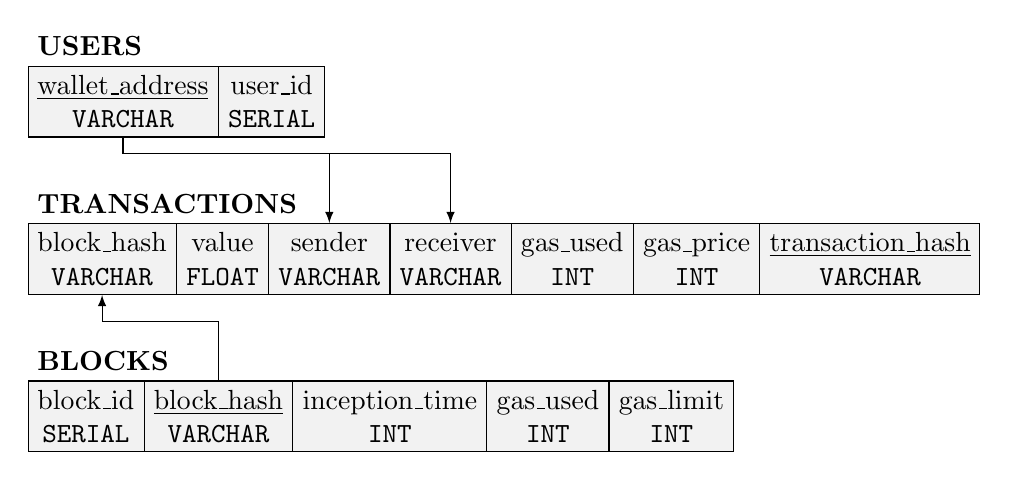
\begin{tikzpicture}[relation/.style={rectangle split, rectangle split parts=#1, rectangle split part align=base, draw, anchor=center, align=center, text height=3mm, text centered}]
% Relations

\node (usertitle) {\textbf{USERS}};

\node [relation=2, rectangle split horizontal, rectangle split part fill={lightgray!50}, anchor=north west, below=0.7cm of usertitle.west, anchor=west] (users)
{\underline{wallet\_address} \\ \texttt{VARCHAR}
\nodepart{two}   user\_id \\ \texttt{SERIAL}};

\node [below=1.3cm of users.west, anchor=west] (transactionstitle) {\textbf{TRANSACTIONS}};;

\node [relation=7, rectangle split horizontal, rectangle split part fill={lightgray!50}, below=0.7cm of transactionstitle.west, anchor=west] (transactions)
{block\_hash \\ \texttt{VARCHAR}
\nodepart{two}     value \\ \texttt{FLOAT}
\nodepart{three}   sender \\ \texttt{VARCHAR}
\nodepart{four}    receiver \\ \texttt{VARCHAR}
\nodepart{five}    gas\_used \\ \texttt{INT}
\nodepart{six}     gas\_price \\ \texttt{INT}
\nodepart{seven}   \underline{transaction\_hash} \\ \texttt{VARCHAR}};

\node [below=1.3cm of transactions.west, anchor=west] (blockstitle) {\textbf{BLOCKS}};

\node [relation=5, rectangle split horizontal, rectangle split part fill={lightgray!50}, below=0.7 cm of blockstitle.west, anchor=west] (blocks)
{block\_id \\ \texttt{SERIAL}
\nodepart{two}        \underline{block\_hash} \\ \texttt{VARCHAR}
\nodepart{three}      inception\_time \\ \texttt{INT}
\nodepart{four}       gas\_used \\ \texttt{INT}
\nodepart{five}       gas\_limit \\ \texttt{INT}};

% Foreign keys

\draw[-latex] (users.one south) --++ (0, -0.2) -| (transactions.three north);
\draw[-latex] (users.one south) --++ (0, -0.2) -| (transactions.four north);
\draw[-latex] (blocks.two north) --++ (0, 0.75) -| (transactions.one south);
\end{tikzpicture}
\caption{Database Model: the primary keys of each table are underlined, foreign keys are represented by arrows, the type of each column is capitalized.}
\label{datamodel}
\end{figure*}


In order to access the data in any form of blockchain technology one must first be an owner of a full node of the respective network. 
This means that the whole blockchain data with all its records is stored on the researcher's device.
An overview of the information stored in the Ethereum blockchain is given in figures \ref{blocks} and \ref{transactions}.
However for the most part, data in this form is not stored in a manner that is easy to query. 
For this reason we opted to become owners of a full node of the Ethereum blockchain, to subsequently scrape the blockchain for the desired information and to store the results in a relational database, which in turn is easy to query.

The data-scraper is written in the \texttt{Python} language using the \texttt{web3.py} module \cite{Python, web3}.
Through \texttt{web3.py}'s interface it is possible to interact with the Ethereum blockchain. 
In particular the \texttt{web3.py} module enables us to extract information for every block and each transaction that is recorded in the blockchain.

In particular, for each block inside a predetermined range we query its contents and obtain the data that is interesting for the further analysis. 
On the block level we extract the hash of each block as a unique identifier and the time each block was inserted into the blockchain. 
Note that this is not necessarily the time that the transaction was being commissioned. 
Finally we query the total gas that was used for each block as well as the gas limit for each block. 
Along with that information we retrieve a list of transactions that are contained within that block.

Making use of the list of transactions within a block we extract the wallet addresses of both sender and receiver, as well as the total value, of the transaction. 
Additionally we retrieve information on the gas price for the transaction. 
Figure \ref{datamodel} summarizes the relations within that database and Algorithm \ref{etl} gives an outline of the datascraper in pseudocode.


\begin{algorithm}
\begin{algorithmic}
\State Check progress file if the ETL can be resumed from a block.
\If {yes}
    \State current block $c \gets$ content of progress file
\Else
    \State $c \gets 1$
\EndIf
\State $s \gets 2000000$ 
\While {$c \leq s$}
   \State Overwrite progress file with $c$ 
   \State $content_{Block} \gets \texttt{getBlock(c)}$
   \State $row_{Block} \gets \texttt{extractInfo(}content_{Block}\texttt{)}$
   \State $\texttt{write(} row_{Blocks}, \texttt{"Block")}$
   \For {each $transaction$ in $content_{Block}$}
       \State $row_{Transaction} \gets \texttt{extractInfo(}transaction\texttt{)}$
       \State $\texttt{write(} row_{Transaction}, \texttt{"Transactions")}$
   \EndFor
\EndWhile
\end{algorithmic}
\caption{Data Scraper: Overview}
\label{etl}
\end{algorithm}


\subsection{Graph Analysis}
We can characterize a network by a number of metrics. The degree of a node in the network is the number of incoming or outgoing edges. We define a \emph{triplet} $i, v, j$ as an ordered set of three nodes, where $v$ is the focal point and the undirected edges $<i, v>$ and $<v, j>$ form the neighboring edges. A triplet is considered closed, when there are exactly three connections for the three nodes. Three closed triplets form a \emph{triangle} \cite{graphintro}. Additionally, we can define multiple measures to investigate a node's role inside the network.

\subsubsection{Degree Centrality}

The most common centrality measure focuses on counting the number of nodes in it's immediate vicinity. It measures the centrality by counting the number of direct connections to the node. For a network with $g$ nodes, the degree centrality of node $n$ is defined as

\begin{equation}
C_D(n) = \frac{k(n)}{g-1},
\end{equation}

where $k(n)$ denotes the degree of node $n$. The Degree Centrality is normalized by $g-1$ since this is the highest possible degree, a node that is connected to every node in the network other than itself \cite{graphintro}.

\subsubsection{Closeness Centrality}

While the Degree Centrality only takes the adjacent nodes into account, it may be possible that the most central in this sense, i.e. the node with the highest degree, is in fact not close to other nodes in the network. This shortcoming is overcome by the \emph{Closeness Centrality}. It considers the sum of geodesic distances, i.e. the number of edges in the shortest path between two nodes. The Closeness Centrality of a network with $g$ nodes is defined as 

\begin{equation}
C_C(n) = \frac{g - 1}{\sum\limits_{i=1}^g d(n, i)},
\label{closeness}
\end{equation}

where $d(i, j)$ stands for the geodesic distance between node $i$ and $j$ \cite{graphintro}.

\subsubsection{Betweenness Centrality}

So far, all the measures focus heavily on the direct influence of the node in question on others. 
However, two nodes which are not adjacent can also influence each other indirectly through other nodes in the network. 
The \emph{Betweenness Centrality} highlights the nodes that lie most frequently in the connecting path between two nodes. 
For a network with $g$ nodes the Betweenness Centrality for node $n$ is defined by the sum over all geodesic distances that pass node $n$, normalized by the sum of all shortest paths of all pairs of nodes:

\begin{equation*}
C_b(n) = \frac{\sum\limits_{j<k} g_{jk}(n)}{g_{jk}}.
\end{equation*}

Here, $g_{jk}$ denotes the number of shortest paths between two nodes of the netwok and $g_{jk}(n)$ marks the number of shortest paths that pass through node $n$. Since the maximum number of such paths is $$\frac{(g-1)(g-2)}{2}.$$ 
One can thus further normalize:

\begin{equation}
C_B(n) = \frac{C_b(n)}{\frac{(g-1)(g-2)}{2}}.
\end{equation}

\subsubsection{Clustering Coefficient}

In order to account for local structures in graph theory, one uses the \emph{Clustering Coefficient}. 
There is evidence that suggests that the ties between nodes in most real-world networks tend to create tightly knit groups with a relatively high density of connections \cite{graphcluster}. 

There exist two versions of this measure, the \emph{global} and the \emph{local} Clustering Coefficient. 
The global Clustering Coefficient $C_G$ is the number of triangles over the total number of open or closed triplets in the graph. 
This measure can be applied to both directed and undirected networks.

The local Clustering Coefficient for a node $n$ is given by the proportion of links between all adjacent vertices divided by the number of links that could possibly occur between them. 
For a directed graph the in- and outgoing edges have a different meaning and therefore the maximum number of immediately adjacent neighbors of $n$ is $k (k-1),$ where $k$ is the degree of node $n$. 
The neighborhood of a node $n$, i.e. its immediately connected neighbors, is defined as $$N = \{n: e_{ij}\in E \cap e_{ji} \in E\},$$ where $E$ is the set of edges. 

Thus the local clustering coefficient of of node $n$ is given by:

\begin{align}
C_L(n) &= \frac{\text{number of closed triplets centered around n}}{\text{number of triplets centered around n}} \nonumber \\
       &= \frac{|\{ e_{jk}: v_j, v_k \in N \cap e_{jk} \in E \}|}{k(k-1)}. 
\end{align}

In an undirected graph the meaning of in- and outgoing edges is considered identical. 
Therefore if a node $n$ has degree $k$, there could exist a total of $\frac{k(k-1)}{2}$ edges within $n$'s neighborhood.
Thus the local Clustering Coefficient of a undirected network can be defined as

\begin{equation}
C_L(n) = \frac{2\cdot |\{ e_{jk}: v_j, v_k \in N \cap e_{jk} \in E \}|}{k(k-1)}.
\end{equation}

This means that nodes with a high Clustering Coefficient play a large role when relaying information through the network \cite{graphbs}.

\subsubsection{Power Law and the Small World Phenomenon}

The small world phenomenon describes that the size of a network does not have any effect on the size of ties among its nodes. 
This means that the path lengths are characteristically small just like random graphs \cite{graphcluster}.

In a random graph the degree of a node $n$ follows a power law distribution, i.e. we can say:

\begin{equation}
P\left(K(n)=k\right) \propto k^{-\alpha},
\end{equation}

where $K(n)$ is the random variable that describes the degree of node $n$ and $\alpha$ is a constant whose values range between $1.6$ and $3.0$ \cite{Newman2003}. 
This distribution suggests that most nodes will have a low degree, while a small number of nodes will display a large number of connections \cite{powerlaw}.

\subsection{Descriptive Analytics}
We collect the basic descriptive metrics that allow getting the initial insights about the network structure and interactions between nodes.
Part of these metrics describe distributions as well as average, median, minimum and maximum values for:
\begin{itemize}
	\item value of a transaction,
	\item amount of gas used in a transaction,
	\item fee paid for a transaction,
	\item number of transactions per block,
	\item value of transactions per block, etc.
\end{itemize}

Another part follows the changes that happen to the network across time. Those are:
\begin{itemize}
	\item number of transactions over time,
	\item volume of transactions over time,
	\item average fees paid per transaction over time, etc.
\end{itemize}

We associate transactions with individual addresses.
This helps to identify:
\begin{itemize}
	\item major senders and receivers of transactions (both in terms of the number of transactions and monetary value exchanges in these transactions),
	\item net balances of accounts in a studied period of time,
	\item distribution of the net balances across the network,
	\item percentage of wealth accumulated and transacted by major nodes, etc.
\end{itemize}

In order to understand our findings in more detail we try to find out identities of the major nodes using data of the Ethereum scanners such as Etherscan.io, Etherchain.org, Blockchair.com,Bloxy.info, etc.

When relevant (for example in case of transactions-outliers, atypical behavior of nodes, discrepancies in data, etc.) we also consider Ethereum forums, posts and newsfeed in order to get additional information about events and actors that may explain or discard certain findings.

\section{Findings}

\subsection{Data Preparation}
We encountered many difficulties during our attempts at collecting and refining the data. 
At first, we attempted to deploy the data-scraper on a \texttt{RaspberryPi 3} Model B in conjecture with an external HDD hard drive. 
We decided on this option, since it did not require any of us to commit indispensable computing ressources and at that time it seemed to be the most convenient option.

That attempt was, in hindsight, doomed to fail due to the hardware's limitations. 
The problem did not lie in the hardware intensity of the data-scraper in itself, but rather in the inordinate amounts of memory it takes for \texttt{go-ethereum} to synchronize with the Ethereum blockchain. 
The interface to the ethereum blockchain, \texttt{go-ethereum}, is written in a manner that is primarily optimized for mining ether and in order to facilitate the commissioning of transactions and smart-contracts. 
The way the programm achieves this is by consuming as much memory as there is available on the system, or at least as much memory as the user is willing to allocate to it before starting the program. 
However, whenever the program runs out of memory or whenever it attempts to exceed its predetermined limit the process shuts down and kills itself. 
This does not result in a system crash, but it does inhibit the workings of the \texttt{Python} libraries that are used inside the data-scraper.

This design of the \texttt{go-ethereum} program frequently led to the \texttt{RaspberryPi}'s 1 GB of memory being filled after only a short period of time, usually between thirty minutes and three hours. 
Note, that the data-scraper's construction did anticipate interruptions and it is possible to resume scraping the Ethereum blockchain from the current block without the loss of any data and without the need to redundandly query more than the one block at which the disconnection happened. 
This behaviour meant that the \texttt{RaspberryPi} was idling for most of the time.

Unfortunate as this was, it was not the only problem. 
The use of an external hard disk drive for storing the database meant that a considerable amount of the time during which the \texttt{RaspberryPi} was productive was spent on input/output-operations while it was commiting the scraped information into the database. 
In order to alleviate the bottleneck that was presented by the I/O-operations it would have been favorable to use an external solid state drive for that task. 
However, we were too frugal to obtain one just for the singular purpose of this seminar paper.

This means that after running the data-scraper for an entire month, along with taking all the care that is reasonable, in order to keep the scraper afloat, we were able to extract 120.000 transactions from 15.000 blocks which tantamounts to merely three days of data.

We solved all these problems by taking up the offer \emph{Microsoft Azure} provides for students. 
Using this free initial student credit on the \emph{Microsoft Azure} servers it was possible to set up a virtual machine with 32 GiB of memory along with access to an additional solid state drive. 
The fact that it is possible to rent out a \texttt{Linux} machine on the \emph{Microsoft Azure} servers made it possible to migrate the scripts for the data-scraper without the need for adjustments.

\begin{table}[ht]
\centering
\caption{Summary statistics}
\begin{tabular}{lrrr}
\toprule
{}    &       value &    gas used &     gas price \\
\midrule
mean  &       48.12 &   127511.76 &  3.01e+10 \\
std   &     1495.49 &   239571.52 &  1.34e+13 \\
min   &        0.00 &    21000.00 &  0.00     \\
25\%  &        0.06 &    40000.00 &  2.00e+10 \\
50\%  &        0.89 &    90000.00 &  2.00e+10 \\
75\%  &        1.11 &    90000.00 &  2.50e+10 \\
max   &  1000000.00 &  4712388.00 &  3.62e+16 \\
\bottomrule
\end{tabular}

\label{summarystats}
\end{table}

The initial student credit was enough to deploying the data-scraper on the \emph{Microsoft Azure} servers for about a week. 
During this week we were able to extract 2 GB of data that consist of one million blocks with a total of 7.3 million transactions made from 415000 distinct wallets. 
Table {\ref{summarystats}} describes some rudimentary statistics.

Initially we also planned to scrape the IP-addresses of a wallet by making use of \texttt{web3.py}'s functionality which is provided for the \texttt{Bitcoin} blockchain. 
However, within the scraped dataset we were not able to identify a single address.
The reason might that the \texttt{web3.py} module does not provide that functionality for the Ethereum blockchain in its current version.
Mind you that we do not claim that it is impossible to retrieve the IP-address of a wallet. 
One proposed heuristic to do so is to assume that the first node that propagates a transaction through the network is also the one that is initializing the transaction \cite{reid2013analysis}. 
However, for us this would have meant to rewrite the data-scraper from \texttt{Python} into the \texttt{Go} language, which we considered to be out of this analysis' scope.

\subsection{Graph Analysis}
\begin{figure*}[t]
\caption{Network Overview}
\centering
\begin{subfigure}[b]{0.5\textwidth}
\centering
\includegraphics[height=155px]{../pics/distribution.png}
\caption{Distribution of total number of transactions}
\end{subfigure}%
\begin{subfigure}[b]{0.5\textwidth}
\centering
\includegraphics[height=168px]{../analysis/centrality.png}
\caption{Centrality Distribution}
\label{centralitydist}
\end{subfigure}
\end{figure*}

Looking at the rough outline of the observed period revealed that almost half of the wallets take part in one transaction during that time frame.
Roughly 16 percent of the wallets appear two or three times respectively.

Since the vast majority of accounts only seem to appear once inside the whole dataset we concluded that these are not interesting from a graph analysis perspective. 
Therefore we opted to use a subset from that data of accounts, where we could verify that they are interacting with other accounts. 
This subset consists of roughly four and a half million transactions in which 27.000 distinct wallets were either the sender or the receiver. 
From this subset we opted to create a graph in which the wallets are represented by the graph's nodes and the transactions are symbolized by the graph's edges.

Even this subset proved to be too large to handle, which means for the further graph-analysis that we were forced to rely on a random subset. 
However, if this random sample is large enough it should still give us an insight into the structure of the Ethereum network and the graph formed by this subset should still provide interpretable results.

\begin{figure*}[!ht]
\centering
\includegraphics[scale=0.475]{../analysis/graph-subsample-1000.png}
\caption{Graph formed by a subsample of 1000 randomly drawn wallets}
\label{graphgraph}
\end{figure*}

\begin{table*}[!ht]
\centering
\caption{Centrality Distribution}
\begin{tabular}{lcccc}
\toprule
{} &  Degree centrality &  Betweenness centrality &  Closeness centrality &  Local clustering \\
\midrule
mean &             0.0001 &                  0.0001 &                0.1540 &            0.0043 \\
std  &             0.0012 &                  0.0020 &                0.0782 &            0.0636 \\
min  &             0.0000 &                  0.0000 &                0.0000 &            0.0000 \\
25\%  &             0.0000 &                  0.0000 &                0.1522 &            0.0000 \\
50\%  &             0.0000 &                  0.0000 &                0.1876 &            0.0000 \\
75\%  &             0.0000 &                  0.0000 &                0.2072 &            0.0000 \\
max  &             0.1344 &                  0.2149 &                0.2862 &            1.0000 \\
\bottomrule
\end{tabular}

\label{graphtable}
\end{table*}

\begin{figure*}[!ht]
\centering
\includegraphics[width=\textwidth]{../analysis/power-law-fit.png}
\caption{Comparison with random graphs}
\label{powerlaw}
\end{figure*}


Figure \ref{graphgraph} displays the graph built from a random subsample of 1000 transactions, where again the nodes represent the different wallets and the edges stand for an observed transaction between them. 
The size of the node stands for the transaction's value. We can clearly see that most of the accounts form connections that consist of only two wallets and it is highly likely that these are also the accounts which are only observed once in the entire dataset. 

Even here it is possible to see that there are subclusters of highly connected nodes associated with a high transaction value located in the middle of the graph. 
This appears despite the small sample size, which has to mean that these nodes in the center of the graph are important actors inside the network whose position will most likely become more pronounced the larger we choose the sample size to be. 
From this first glimpse{\parfillskip0pt\par}

\noindent at the network we would expect to find two tendencies inside the dataset. 
First, we expect a large number of nodes which are associated with low centrality measures and clustering coefficients. 
Secondly we expect to find some collections of nodes that form subgroups and within these subgroups we should be able to locate some nodes that play a tangible role in their respective local neighborhoods. Both of those observations do fit into the notion of a random graph, where we would expect a large number of loosely connected nodes with a low degree and an exponentially lower quanity of nodes which have a higher degree and who play a more central role inside the network.

Note nonetheless, that figure \ref{graphgraph} provides only a rough outline since it is only using one thousand out of the 7.3 million available transactions. 
We pick a comparatively small sample size for this graph in order to avoid overplotting, the further analysis however uses a larger subsample of 100000 transactions.

The results of the larger subsample are summarized in table \ref{graphtable} and figure \ref{centralitydist}. 
For the Degree Centrality we can observe a highly skewed distribution, where the mean lies at $\bar{C_D} = 0.0001$, whereas the first three quartiles remain firmely at $0$. 
This indeed confirmes our previous suspicion that most nodes inside this network are merely loosely connected, even after removing the most isolated and remote nodes of the initial dataset. 
This means that most wallets interact only with are very limited set of other wallets and that it is highly uncommon for a node to accept transactions from many different wallets.

When looking at the results for the graph's Betweenness-Centrality, we can see a similiar pattern. 
The mean lies at $\bar{C_B}=0.0001$ and all three quartiles are, again, $0$. This means that the Betweenness centrality's distribution is also heavily skewed, which indicates that only a few nodes act as a mediator for their neighbors. 
This should not come as a surprise, since most of the nodes have a very low degree to begin with.

The Closeness centrality between all nodes paints a different picture. Its distribution is still skewed, however it is not as extremely skewed as the measures that have been discussed so far. 
The mean lies at $\bar{C_C}=0.15$ with a standard deviation of $s_{C_C} = 0.078$. 
Note that this measure needs to be interpreted with care. 
Most of the nodes are disconnected, and thus do not have a connecting path at all. 
If a node $j$ cannot be reached from a different node $k$ there exist two common propositions in the literature. 
Either $d(j, k) = 0$ or $d(j, k)=\infty$. 
Most implementations rely on the former convention rather than the latter, since it avoids values that cannot interpreted as a number. This is also the convention that is implemented in the \texttt{networkx} module for the \texttt{Python} programming language \cite{networkx}. But this also means that the closeness centrality should be interpreted as a local measure since the distances in the normalizing factor in (\ref{closeness}), which are calculated as $$\sum\limits_{i=1}^g d(n, i),$$ will contain numerous zero-valued summands. So actually, this measure only makes sense for nodes that are of a degree $k$ that is larger than three, since nodes of a lesser degree are necessarily close to each other.

The Local clustering coefficient accross the nodes is again highly skewed to the left. The mean lies at $\bar{C_L}=0.004$ at a standard deviation of $s_{C_L}=0.063$. Again the quartiles are all planted at $0$. Note however, that there exist some nodes whose Local clustering coefficient reaches as far as $C_L(n)=1$. This means that there are some nodes who are fully connected within their local cluster, which means that all triangles within that clique are centered around that node $n$. This, in turn, means that there are some nodes which are perfectly connected inside their neighborhood.

So far all these findings indicate that the model of a random graph would be a good approximation of the real world data. In order to test this assumption in a graphical manner, we would like to compare the empirical density functions of the degrees against the theoretical powerlaw distribution. Remember that, in a random graph, the random variable $K(n)$ that describes the degree of a node $n$ follows a powerlaw distribution $$P(K(n)=k)\propto k^{-\alpha},$$ where $\alpha$ is some constant that has to be determined by Maximum-Likelihood methods \cite{graphintro}. Figure \ref{powerlaw} presents the results for the empirical probability density function (PDF) and the complementary cumulative distribution function (CCDF). The CCDF is primarily used in the domain of signal processing and measures the the amount of time a signal spends above the mean power level of the measured signal. Equivalently, it assesses the probability that the signal power will be above the average power level \cite{ccdf2015}.

In order to reflect the difference in the roles accross the network such as the reciever or the sender of a transaction, we split the analysis into three different parts. First, we look at the distribution of the directed graph that is focusing on the actors that iniatate a transactions, i.e. the senders. Second, we look at the network formed by the receivers of a transaction and finally we look at the whole undirected graph that contains both receivers and senders. The results are displayed in figure \ref{powerlaw}. The PDF is shown by the blue line and the CCDF is represented by the red line. A high overlap between the dashed and the solid line indicates a good fit of the empirical distribution compared to the theoretical. Thus the probability density function of a perfectly random network would lie on its respective dashed line.

In the leftmost part of figure \ref{powerlaw} we can see for the senders that the tails of the empirical PDF are closely following the theoretical distribution of the random graph. However, in the central part we observe one large deviation from the distribution of a random network. In particular, this means that - under a random graph - we would have expected more nodes that have a middling degree, i.e. $k=3$, $k=4$, and so forth. Instead, we observe a large number of loosely connected nodes.

The same holds for the sender's CCDF. The lower tail of the distribution follows the random graph closely, whereas the central part is too low, and the upper tail is too high for a random graph.

Looking at the wallets at the receiving end of a transaction, in the middle part of figure \ref{powerlaw}, we can discern a similar pattern. Both, the line for the PDF, as well as the line for the CCDF begin by closely following the theoretical distribution and begin to deviate after passing the median. Again we observe a density at the lower tail that is very similar to what we would expect from a random graph.

However, the most clear indicator of that pattern is shown for the composite graph, that contains both senders and receivers, in the rightmost part of figure \ref{powerlaw}. Here we observe a very pronounced deviation from the course of both the theoretical PDF and CCDF after reaching the median. Again, this is a clear indicator that there are too many nodes with a comparatively high degree, for this to be a random network.



\subsection{Descriptive Analytics}
Descriptive analysis of the data allows getting insights that can be useful at the time of the network analysis.
By itself alone it can point at important information with regard to the network structure, interactions between the nodes, underlying business processes, design problems, potential privacy and security issues.

For instance, while the median value of a transaction is equal to 0,9 ether, the value of the biggest one is 1 million ether (138 million U.S. dollars as of 15.03.2019). 
Figure \ref{fig:value_per_tx} shows the distribution of value sent in individual transactions. 
There is a significant number of outliers indicating at certain concentration of ether holdings.


\begin{figure}[h]
  \centering
  \includegraphics[width=\linewidth]{figures/value_per_tx.jpeg}
  \caption{Distribution of Value sent per Transaction.\\ 
  \textit{*The number of transactions on the Y axis is limited to 50, so that the less frequent values remain visible.}}
  \label{fig:value_per_tx}
\end{figure}

The amount of fees paid in transactions gives a hint at the underlying variation in businesses activity and Ethereum design issues. 
Cryptocurrencies are often promoted as a fast medium for micro-payments. 
However, fast transactions with low fees are not always the case.
Limitations in the block size and the number of blocks in a period of time may result in an overflow of transactions pending to be included in a block.
To speed up transactions people pay higher fees.
At the same time, when the exchange rate of a cryptocurrecny rises, fees tend to become lower.

\begin{figure}[h]
  \centering
  \includegraphics[width=\linewidth]{figures/fee_per_tx.jpeg}
  \caption{Distribution of Fees paid per Transaction.\\ 
  \textit{*The number of transactions on the Y axis is limited to 700, so that the less frequent fees remain visible.}}
  \label{fig:fee_per_tx}
\end{figure}

Interestingly, the is a big outlier - once there was a fee of more than 600 ether (80 000 U.S. dollars as of 15.03.2019).
Apparently this is due to a mistake made by a payer.
Such a mistake shows one of the disadvantages of the blockchain-based currencies where all transactions are irreversible.

Analysis of the distribution of gas used in transactions (see Figure \ref{fig:gas_per_tx}) points at differences in their types.
As gas measures how much "work" an action or a set of actions takes to perform, this potentially can be used to make a preliminary judgement about the prevalence of the smart contracts or about distribution of their complexity.

\begin{figure}[h]
  \centering
  \includegraphics[width=\linewidth]{figures/gas_per_tx.jpeg}
  \caption{Distribution of Gas used per Transaction. \\ 
  \textit{*The number of transactions on the Y axis is limited to 70 000, so that the less frequent amount of gas remain visible.}}
  \label{fig:gas_per_tx}
\end{figure}

There are obviously two major clusters that probably separate regular payment transactions and smart contracts plus several groups of more complex contracts that however represent minority in the total volume of transactions. 
Both median and the 3rd quartile amount of gas is equal to 90 000 wei. In case the above hypothesis is correct, regular payment transactions will cover at least 75 \% of the total number and are all represented on the Figure \ref{fig:gas_per_tx} by the 1st bar (cut in order to make other values visible).

Analysis of the transactions number over time makes the concern about unequal distribution of wealth in the network visible. 
As illustrated on the Figure \ref{fig:tx_over_time} the number of transactions on the most active days more than doubles the respective number on the days with the lowest activity. 
Such significant variation indicates at the presence of major nodes.  

\begin{figure}[h]
  \centering
  \includegraphics[width=\linewidth]{figures/tx_over_time.jpeg}
  \caption{Number of Transactions over Time.}
  \label{fig:tx_over_time}
\end{figure}

This becomes even more visible if we consider the monetary volume of transactions over time (see Figure \ref{fig:volume_over_time}).
Increases in volume of up to a hundred times from one day to another are an example of activity that would lead to a drastic changes in prices if these transactions are made not on chain but on currency exchanges.

\begin{figure}[h]
  \centering
  \includegraphics[width=\linewidth]{figures/volume_over_time.jpeg}
  \caption{Volume of Transactions over Time, in ether.}
  \label{fig:volume_over_time}
\end{figure}

\begin{figure*}[h]
  \centering
  \begin{subfigure}[b]{0.49\linewidth}
    \includegraphics[width=\linewidth]{figures/major_receivers_metrics.jpeg}
    \caption{Top 50 Receivers.}
    \label{fig:major_receivers_metrics}
  \end{subfigure}
  \begin{subfigure}[b]{0.49\linewidth}
    \includegraphics[width=\linewidth]{figures/major_senders_metrics.jpeg}
    \caption{Top 50 Senders.}
    \label{fig:major_senders_metrics}
  \end{subfigure}
  \caption{Cumulative Percentage of Transactions (blue) and Volume (orange) covered by Major Receivers (a) and Senders (b).}
  \label{fig:major_metrics}
\end{figure*}

In order to verify the hypothesis about the presence of major nodes we analyse transactions number and volume more in depth. 
This is done by associating transactions with individual accounts.
We treat receivers and senders of transactions separately.

As shown on the Figure \ref{fig:major_receivers_metrics} top 5 major accounts have received 19,9 \% of all transactions (1,45 out of 7,3 million transactions).
Top 50 accounts cover slightly more than one third of the total transactions' number.
When it comes to the monetary value, the situation is even more centralized.
Top 5 accounts have received 31,8 \% of the total transactions' value (112 out of 352 million ether received in all transactions).
Major 50 Receivers cover more than a half of the volume transacted within the network. 

Figure \ref{fig:major_senders_metrics} shows the data for major senders of transactions.
Here, in terms of the transactions' number the situation is even more centralized.
Top 5 accounts have made 36,4 \% of all transactions.
Top 50 senders cover 60,1 \% of the entire transactions' number.
At the same time in terms of volume the picture is different.
Top 5 and Top 50 senders cover only 18,3 \% and 35,0 \% of the total transactions' value respectively.

Interestingly, there are significant discrepancies in the degree of centralization if the data about receivers and spenders is compared to each other.
This is the case for centralization both in terms of transactions' number and volume.
Analysis of these discrepancies may shade light on some of the roles that major nodes play in the network.

\textit{Discrepancies in the Transactions' Volume between Receivers and Senders.} 
There is a significant difference between the amount of ether received and spent by the major accounts.
While Top 50 Receivers have accumulated 172 million ether, Top 50 Senders have spent only 123 million.
Besides, top receivers and senders should not necessarily be the same entities. 
Consequently there is a number of major nodes that spend less than their receive or don't spend at all.
Figure \ref{fig:balances} shows the net balances of the accounts within the studied period of time. 
While absolute majority of accounts have balance around 0, there are few that have accumulated a significant amount of wealth.

\begin{figure}[h!]
  \centering
  \includegraphics[width=1\linewidth]{figures/balances.jpeg}
  \caption{Distribution of Balances within Studied Period. \\ 
  \textit{*The number of wallets on the Y axis is limited to 10, so that the less frequent wallets remain visible.}}
  \label{fig:balances}
\end{figure}

Those could be mining pools that receive new coins and hold them anticipating appreciation of ether.
However the amount of Ethereum accumulated by such nodes seems to be too big to be explained this way.
Despite a new block in Ethereum is mined every 10-20 seconds and remunerates miners with 5 ether, during the analyzed period of time this results in only approximately 5 million new ether.

Probably, these nodes are currency exchanges that accumulate wealth of their participants. 
They keep track of exchange transactions internally without recording them on-chain. 
The wealth is recorded as spent only when a participant makes a payment transaction.

If the nodes are actually currency exchanges, there is a deviation from the Ethereum narrative of "no trusted third party involvement".
Given the level of centralization associated with the nodes, this could imply a major source of vulnerability.
An attack on the exchange records would lead to losses for a significant number of the exchange participants.

\begin{table*}
\centering
\captionof{table}{Top 5 Major Receivers (Volume)} 
\label{tab:t5mr} 
\begin{adjustbox}{width=0.9\linewidth}
% \small
% \resizebox{\columnwidth}{!}{%
\begin{tabular}{lccl}
% \begin{tabulary}{\linewidth}{RLRR}
  \hline
Wallet & Amount Received, mill. ether & Type & Affiliation \\
  \hline
  0xAA1A6e3e6EF20068f7F8d8C835d2D22fd5116444 & 66,0 & Smart-Contract & ReplaySafeSplit \\ 
  0xBFC39b6F805a9E40E77291afF27aeE3C96915BDD & 13,2 & Smart-Contract & Poloniex \\ 
  0x209c4784AB1E8183Cf58cA33cb740efbF3FC18EF & 12,6 & Smart-Contract & Poloniex 2 \\ 
  0x7727E5113D1d161373623e5f49FD568B4F543a9E & 11,1 & Smart-Contract & Bitfinex 2 \\ 
  0xFa52274DD61E1643d2205169732f29114BC240b3 & 8,5 & Smart-Contract & Kraken 4 \\ 
   \hline
% \end{tabulary}
\end{tabular}
\end{adjustbox}
% }
\end{table*}

\begin{table*}
\centering
\captionof{table}{Top 5 Major Senders (Number of TXs)}
\label{tab:t5ms}
\begin{adjustbox}{width=0.9\linewidth}
\begin{tabular}{p{7cm}ccl}
  \hline
Wallet & Number of TXs send & Type & Affiliation \\
  \hline
  0xEA674fdDe714fd979de3EdF0F56AA9716B898ec8 & 733818 & Address & Ethermine \\
  0x2a65Aca4D5fC5B5C859090a6c34d164135398226 & 715017 & Address & DwarfPool 1 \\
  0xD34DA389374CAAD1A048FBDC4569AAE33fD5a375 & 516932 & Address & GenesisMining \\
  0x52bc44d5378309EE2abF1539BF71dE1b7d7bE3b5 & 443544 & Address & Nanopool \\
  0x61C808D82A3Ac53231750daDc13c777b59310bD9 & 251566 & Address & F2Pool 1 \\
   \hline
\end{tabular}
\end{adjustbox}
\end{table*}

In order to verify how relevant this risk actually is, we conducted further investigation of the accounts that received the biggest volumes of ether.  
Using data of the Ethereum scanners such as Etherscan.io, Etherchain.org, Blockchair.com, Bloxy.info, etc.\footnote{For details see: \\ \url{https://etherscan.io/}, \\ \url{https://www.etherchain.org/}, \\ \url{https://blockchair.com/Ethereum/}, \\ \url{https://bloxy.info/}.} we found out affiliation of the Top 5 Receivers (in terms of volume).

Four out of five Top Receivers actually belong to the currency exchanges (see Table \ref{tab:t5mr}).
However, all these accounts in reality appeared to be not regular addresses but smart contracts.
The remaining Top Receiver (the first one in the list) is also a smart contract.
None of them is supposed to accumulate wealth and by design should transfer it further.
This puts under question the validity or completeness of the transactions´ data we have collected.

Deeper research allowed restoring the faith in the dataset.
Appeared that money received by identified major accounts was actually spent.
Bit in another network.

The point is that on the 20th of July 2016 (shortly before the analyzed period) Ethereum experienced a hard fork.
As a consequence of the DAO incident - a hack of a complicated smart-contract that resulted in a loss of about 12.7 million ether (worth around 150 million U.S. dollars at the time) - the community was split in two parts.
Most of the network participants decided to make a fork chain where the stolen coins would be returned to their owners.
However, some of the community decided to continue the old chain (Ethereum Classic or ETC), arguing that "the code is the law" and the blockchain data should be irreversible\footnote{See for instance \url{https://www.cryptocompare.com/coins/guides/the-dao-the-hack-the-soft-fork-and-the-hard-fork/}.}.

This lead to a number of issues related to the interaction between chains.
One of the most relevant of them was "replay attack".
The mechanics of it is as follows:
if there is a valid transaction on one chain, it can also be offered - replayed - on the other chain to duplicate the received amount.
For instance, a user of the currency exchange can deposit and withdraw her money from this exchange on the old chain, and then use the 2nd transaction to withdraw money also on the new (forked) chain\footnote{See for instance \url{https://vessenes.com/hard-fork-and-replay-concerns/}.}.
This concern was solved through inter-mediation of the smart contracts.
Thus, the post by Ethereum founder Vitalik Buterin states:
"users who are interested in taking any actions with their ETC, including creating and participating in applications, converting to another asset, etc. are advised to use the splitter contract at address 0xAA1A6e3e6EF20068f7F8d8C835d2D22fd5116444 to move their ETC to a separate newly created account so as to avoid replay attacks; we also encourage the ETC community to consider adopting a secondary hard fork to change transaction formats to make further replay attacks impossible\footnote{For details see \url{https://blog.Ethereum.org/2016/07/26/onward_from_the_hard_fork/}.}.

The address mentioned in the post is the biggest Receiver in our dataset\footnote{The original address in the post was substituted as the original smart-contract was changed.}.
It has transmitted all the received money to its senders, but on the other chain.
The other 4 accounts, which are intermediate exchange wallets were apparently performing similar function of splitting wealth between different chains.

Thus, our concern about possible attack is confirmed only partially.
None of the Top 5 Receivers were accumulating wealth and it all was automatically transmitted to other accounts.
At the same time while exploring the "ReplaySafeSplit" smart-contract we have found that a number of users lost their money due to the mistakes made by them during the split\footnote{See for instance \url{https://medium.com/@chevdor/safer-version-of-the-replaysafesplit-smart-contract-a29c347e8a7}.}.
The smart-contract itself appeared to be susceptible to a number of bugs\footnote{For details see \url{https://etherscan.io/address/0xaa1a6e3e6ef20068f7f8d8c835d2d22fd5116444\#code}.} and was later substituted by another one.
The DAO incident described in the context of our Receivers exploration also exemplifies how the risk of the attack on an account or contract that holds funds from different users can and has actually played out.

\textit{Discrepancies in the Transactions' Number between Receivers and Senders.} 
As has been described by the Figure \ref{fig:major_metrics} the number of transactions received by major Receivers is significantly smaller than the number of transactions made by major Senders.
This discrepancy can probably be partially explained by the activity of the mining pools.
There, one account receives a mining reward and then sends it in small fractions to the many participants of the pool.

Alternative explanation can be related to various approaches of the network participants to gain more privacy.
One of them is the so called "peeling-chain".
The technique consists in dividing and sending the wealth of an account to multiple addresses again and again.
The goal is to create an impression that several users are doing transactions instead of one.

The process is illustrated on the Figure \ref{fig:peeling_chain}.
Here, the received amount of 50 coins is splitted in several iterations to multiple accounts in an attempt to complicate tracking of a certain person´s wealth.

\begin{figure}[h]
  \centering
  \includegraphics[width=\linewidth]{figures/peeling_chain.png}
  \caption{How the peeling-chain works. \\
  \textit{From \cite{balthasar2017laundary}}}
  \label{fig:peeling_chain}
\end{figure}

Further research of the Top 5 transaction Senders allowed verifying the hypotheses about the role of different nodes and their activities.
Using data of the Ethereum scanners as before we disclosed identities of the major accounts. 
All of them appeared to be mining pools (see Table \ref{tab:t5ms}.
Among Top 5 Receivers of transactions there are no mining pools (the accounts are a digital token YoCoin, 2 Poloniex exchange wallets, currently closed by the U.S. government cryptocurrency trading platform BTC-e and already mentioned ReplaySafeSplit smart-contract).
Thus the hypothesis about the activity of mining pools is confirmed.
"Peeling-chain" practices are neither confirmed nor disproved.

% Accounts receiving major number of transactions were rarely (only ..times) seen in the list of major senders





% \begin{figure}
%   \centering
%   \includegraphics[width=\linewidth]{figures/volume_per_block.jpeg}
%   \caption{Distribution of Transactions' Volume per Block.}
%   \label{fig:volume_per_block}
% \end{figure}



\section{Conclusion}
This work aimed to transfer the approaches of the Bitcoin paper \cite{lischke2016analyzing} to the Ethereum blockchain and to get some insights about the underlying Ethereum economy and network. 
To do so, transaction data for 6 months got scraped, displayed and analyzed.

Eventually, we replicated some of the approaches suggested in \cite{lischke2016analyzing}, adopted the others, or came up with new approaches due to the differences in the design and supporting infrastructure of the Ethereum and Bitcoin blockchains.

Beforehand, we looked into the previous studies of Ethereum blockchain to gain a better understanding of what was done so far, to benefit from existing findings and potentially to identify the blank spots.
% and might find additional information about how to get good off-set data or IP addresses.
Although Ethereum is relatively new, some articles have been published that have already dealt with the address space, security aspects and theoretical aspects of the Ethereum network.
We identified 4 categories of papers dedicated to the topic.
The papers focused on descriptive analysis and network metrics analysis appeared to be less present.
Therefore, we have combined these two categories in our research and used relevant papers as an inspiration when amending approaches of \cite{lischke2016analyzing}.

% None of them brought together transaction and network data to analyze patterns in the combined offset and network data over an extended time period.

% With that knowledge we worked our way through the same platforms, 'bitcoin.info' to enrich our data set and analyze it in the descriptive and graph analysis.

Descriptive analysis delivered information about the network structure and interactions between the nodes.
Thus, the data showed that the transactions volume was varying over time with sudden increases of up to a hundred times.
This gave the impression that there are major nodes, which distribute disproportional amounts of Ether in the network.
Further analysis revealed that the Top 5 Senders perform 36\% of the transactions in the network.
If the Top 50 Senders are considered, the network is even more centralized - 60,1\% of all transactions are covered by them.
Top 5 and Top 50 addresses received 32\% and 50\% of the monetary volume transmitted within the network.
Our findings are consistent with those of \cite{payette2017characterizing} who identify 4 behavior clusters of different network participants.

Although we were not able to get data about the IP addresses and business tags for all the transactions in the data set, we did discover the identities of the most active network participants.
This helped to shed the light on the underlying business processes that are relevant for a significant part of the network.
For instance, through online research, we have shown that the top 5 transaction Senders can be identified as mining pools.
We also found out that the 4 main Receivers (in terms of volume) are associated with currency exchanges.
All of them appeared to be smart contracts, as well as the first major receiver. 
These findings are mostly in line with \cite{anoaica2018quantitative} and \cite{chen2018understanding}.
Through online research, we discovered that the biggest receiver is a smart contract ReplaySafeSplit designed to deal with the side effects of the hard fork that happened in 2016. 
This can partly explain the relatively higher importance of smart contracts according to our research and extends the research of \cite{kiffer2017stick}.


While doing descriptive analysis and supportive online research of anomalies, we also spotted signs of design problems, potential privacy and security issues.
Thus, the distribution of fees paid per transaction points at the limited number of transactions that can be transmitted in a period of time.
Accumulation of wealth by major accounts can lead to price manipulation if this wealth is used on currency exchanges.
Major accounts and smart contracts, which accumulate the wealth of many network participants, were found to be prone to bugs and can potentially also be attacked.
The major role of the ReplaySafeSplit smart contract which has received the highest volume of the transactions in the dataset is due to the "replay" attack concerns that arose after the DAO incident and hard fork of the Ethereum blockchain.
The hypothesis about the chain-peeling used to increase the privacy of transactions was neither confirmed nor rejected.

% Due to the fact, that there are major nodes one could identify indirectly the underlying business processes. 
% The discrepancies in the transaction volume could not be investigated conclusively just through the scraped data alone. 


% An alternative hypothesis, which would involve potential privacy and security issues could neither be confirmed nor disproved.

Our findings about the network structure of the Ethereum blockchain were further confirmed, when the distributions of several centrality measures were computed and interpreted. 
Major results are that within the network one can find major hubs with high transaction volume. Most of the nodes are not connected. 
They are usually just having little transactions between each other. 
These findings are in line with \cite{anoaica2018quantitative} and \cite{kim2018measuring}.
The fit with a theoretical power law distribution shows, the \emph{Small World Phenomenon} can only be confirmed for subgraphs within the network.
This is also expected given the fact that the graph analysis found out that there are very little nodes which cover moderate to high amounts of transactions.
Our results partly confirm those achieved by \cite{somin2018network} and \cite{anoaica2018quantitative}.
The discrepancies can be due to the smaller subset of data we used.

Originally the Ethereum protocol was thought of as a modified version of the Bitcoin Blockchain. 
That's what Vitalik Buterin had in mind when he wrote the white paper in 2014. 
The turing completeness should provide opportunities to create applications for any type of application \cite{vitalikwhite}.

Buterin's idea was to optimize the Etherum Blockchain technology to make the blockchain technology more applicable for a larger range of applications. 
He thought Ethereum being open-ended by design and believed that it is extremely well suited to serve as a basic layer for financial and non-financial applications \cite{vitalikwhite}.

As has been shown in the comparison between blockchain and bitcoin, one could guess, that so far this goal is not close to being reached by the Ethereum community. 
There are lots of attempts to create applications for the platform and try to find business cases. 
An indication for that claim is the fact that the number of actively used Ethereum addresses has dropped below 1 million and also that a study on the usage of smart contracts indicated, that 95\% are used just less than 10 times and only 5\% more than that \cite{Chandersekhar2018}. This is also in line with our findings made during descriptive analysis.
An interesting question would be, how many contracts exist that are just using up computational capacity without being used more than a few times.

To conclude, performed analysis of Ethreum blockchain deviates to a certain extent in its approaches from those suggested by Lischke and Fabian.
However, it still seems to extend the understanding of the Ethereum blockchain, underlying business activity and interactions between the nodes. 
It also attracts attention to certain design and security issues, confirms part of the findings made by previous researches and poses an urge for further research in the areas where discrepancies are found.

The research had some limitations along the way.
A crucially limiting factors were the access to the different data sets and the amount of data to be collected.
Hopefully, future researches will be able to locate the transactions via IP addresses and collect the business tags not only for the major nodes but for the entire dataset.
% The data was incomplete, and we were not able to locate the transactions via IP addresses. 
% In the replicated paper they were able to scrape the data with the transaction data, using 'blockchain.info'. 
% This is not possible for the Ethereum blockchain and a proper workaround was not found easily. 
% We searched for alternative providers, but none of them gave information about the sender's IP address.
% Thus, we could not trace the sender's geographical location, or find a mapping to the wallet's industry tag either. 
Another challenge is, that the network is, in essence, different from the Bitcoin.
Especially, because the Ethereum blockchain also provides smart contracts in addition to a currency service.
Where the distinction is not easily made in the data.
Some use the platform just for transactions and a lot of them apply smart contracts or decentralized applications.
As mentioned in the methods, for a further paper one could look in more detail into the scraper we applied and modify it for the usage in the 'go' language.
% 
To get back to the data, unfortunately, the time period gathered was immediately after the hard fork which happened in the Ethereum network in July 2016.
% All that happened because of a hard fork incidence, when a complicated hack of a smart contract led to a loss of 12,7 million US Dollar.
% The network got divided and had to reorganize. 
This brought the noise in the data, which is not the usual situation.
To get better and broader explanations, one may use a different or a longer period.
% However, one is also hard-pressed to find a period in the Ethereum blockchain that does not experience heavy turmoil.

\bibliographystyle{apacite}
\bibliography{references}

\end{document}
